\chapter{Abbreviations and reference data}

\section{Basic molecular biology data}

\begin{itemize}
\item     Figure~\vref{fig:aas} shows structures and abbreviations for the
    20 naturally occurring amino acids.  The abbreviations shown in
    the figure are used consistently throughout this thesis.

\item     Figure~\vref{fig:bases} shows structures and abbreviations for the
    four nucleotides found in DNA and RNA, and urysil, which is
    found only in RNA

    \item     Table~\vref{table:codonTable} shows the standard codon table
    that translates from three letter nucleotide sequences to the
    corresponding amino acid during the process of mRNA translation.
\end{itemize}


        \begin{figure}[ptbh]
        \centering
        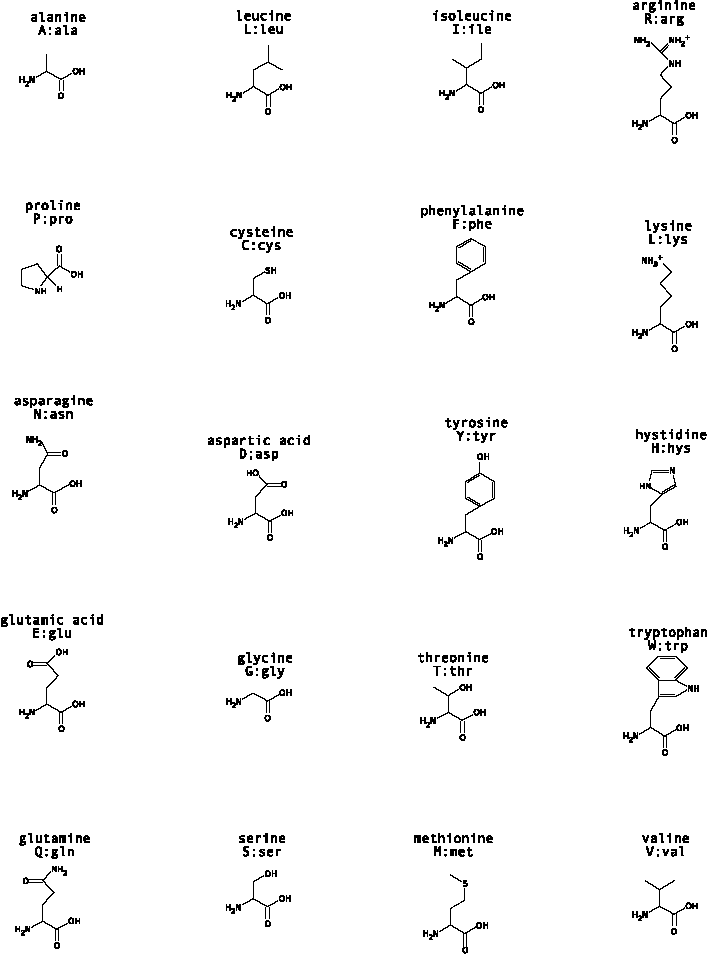
\includegraphics[width=\textwidth]{Body/Images-appa/aas.pdf}
        \caption[Amino acid structures and abbreviations]{Amino acid structures and abbreviations.  The figure shows the chemical
structure of the 20 naturally occurring amino acids and their three letter and
one letter abbreviations.}
        \label{fig:aas} \end{figure}


.
        \begin{figure}[bthp]
        \centering
        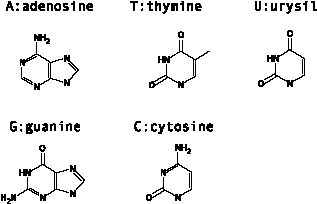
\includegraphics{Body/Images-appa/bases.pdf}
        \caption[Nucleotide base structures and abbreviations]{Nulceotide base structures and abbreviations.}
        \label{fig:bases} \end{figure}



    \begin{table}[tbph]
    \caption[Standard codon table]{Standard codon table.  The table
    should be interpreted by reading the first and second
    nucleotides off of the vertical axis on the left, and reading
    the final nucleotide off of the horizontal axis at the top.
    For example, the amino acid corresponding to the three
    nucleotide sequence \texttt{AAG} is \texttt{Arg}, or arginine.
    }\label{table:codonTable}
    \centering
\begin{verbatim}
                  A      C      G      U
             _____________________________
        AA  |    Lys    Asn    Lys    Asn
   F    AC  |    Thr    Thr    Thr    Thr
   i    AG  |    Arg    Ser    Arg    Ser
   r    AU  |    Ile    Ile    MET    Ile
   s P  CA  |    Gln    His    Gln    His
   t o  CC  |    Pro    Pro    Pro    Pro
     s  CG  |    Arg    Arg    Arg    Arg
   & i  CU  |    Leu    Leu    Leu    Leu
     t  GA  |    Glu    Asp    Glu    Asp
   S i  GC  |    Ala    Ala    Ala    Ala
   e o  GG  |    Gly    Gly    Gly    Gly
   c n  GU  |    Val    Val    Val    Val
   o    UA  |     .     Tyr     .     Tyr
   n    UC  |    Ser    Ser    Ser    Ser
   d    UG  |     .     Cys    Trp    Cys
        UU  |    Leu
\end{verbatim}

    \end{table}


\clearpage

\section{Supplementary data and analyses}

\subsection{Position weight matrix computation and matching}\label{section:pwmCode}

The code shown below is a simple Python script used to compute a
position weight matrix.  The script can be copied from this text and
run on most personal computers.  After the code, I present a brief
example of how this should be run, using the yeast 3' splice sites
shown in Figure~\vref{fig:yeast}.

\begin{singlespace}
\small
\verbatiminput{Body/Images-appa/searchPwm.py}
\normalsize
\end{singlespace}

\begin{singlespace}
\small
\verbatiminput{Body/Images-appa/pwm-run.txt}
\normalsize
\end{singlespace}

\subsection{Antimicrobial design data}

    Figure~\vref{fig:synth1ms} shows the gas and mass spectra for a
    peptide designed in Chapter~\ref{chapter:amps}.  See
    Section~\vref{section:preliminary}.

        \begin{figure}[htbp]
        \centering
        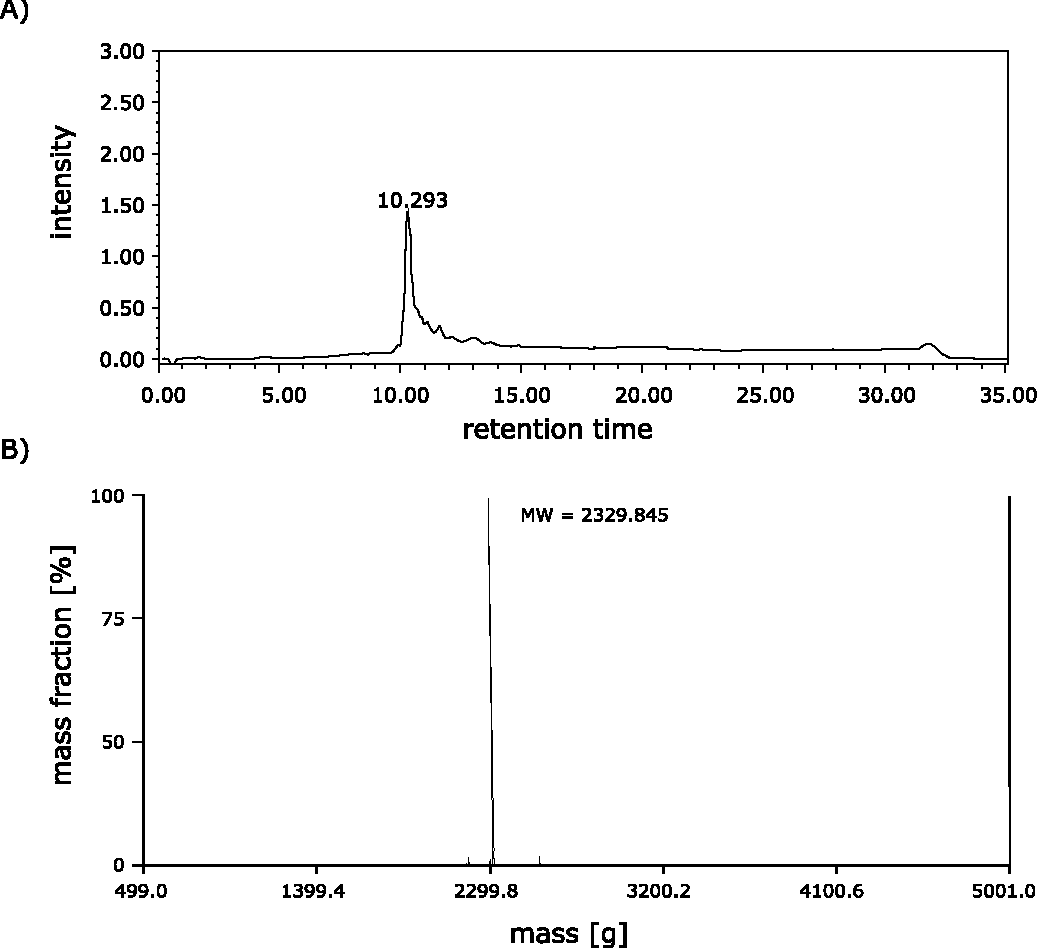
\includegraphics[width=\textwidth]{Body/Images-appa/synth1-spectra.pdf}
        \caption[Gas and mass spectra for the synth--1 peptide]{
        Gas and mass spectra for the synth--1 peptide.  As the
        figure shows, the peptide appears well above  the 85\% purity
        threshold.  This peptide was designed using our preliminary,
        sensitive approach for designing antimicrobial peptides.
        However, the peptide was shown to have undetectable activity
        under good experimental conditions, prompting the more
        focused, specific approach for designing AmPs.
        }
        \label{fig:synth1ms}
        \end{figure}
